\documentclass[11pt,a4paper]{article}
%\documentclass[10pt,twocolumn]{article}


\usepackage{Movements} %% cibler doc/modules/
\setlength{\columnsep}{1cm}


%\onecolumn
\begin{document}
  \fairetitre{Amélioration de la réactivité des réseaux pair à pair pour les MMOGs}{Étude bibliographique sur les déplacements en groupe dans les MMOG}{Xavier Joudiou}{Sergey Legtchenko \& Sébastien Monnet}{10/06/10}

\newpage
%\onecolumn
\tableofcontents
\newpage
%\twocolumn

\noindent{\textbf{Résumé}}\\
	\par \textit{Depuis plusieurs années, un nouveau type d'architecture des systèmes est apparu. Il s'agit de l'architecture pair à pair, cette architecture est devenue populaire grâce à des applications de partage de fichiers. Nous allons nous intéresser aux jeux vidéos massivement multijoueur (MMOG pour Massively Multiplayer Online Games) qui sont de plus en plus populaires et qui font ressortir des problèmes que l'architecture pair à pair doit pouvoir corriger. Le problème du passage à l'échelle sera l'un des plus importants à résoudre pour permettre à un grand nombre de joueurs de participer simultanément. Nous verrons comment l'architecture pair à pair peut être une des solutions.\\ 
	 Pour remédier à cela, une solution consiste à remplacer le modèle client/serveur par un réseau logique pair à pair (overlay). Malheureusement, les protocoles pair à pair existants sont trop peu réactifs pour assurer la faible latence nécessaire à ce genre d’applications. Néanmoins, quelques travaux ont déjà été menés pour adresser ce problème. L’idée est d’adapter le voisinage de chaque pair afin que toute l’information dont il aura besoin dans l'avenir se trouve proche de lui dans le réseau. Il est alors nécessaire de correctement évaluer les futurs besoins de chaque pair, et de faire évoluer son voisinage à temps. Dans ce rapport bibliographique, nous allons étudier les mouvements de groupe et ainsi nous pourrons voir si cette piste est exploitable pour l'amélioration de la réactivité des réseaux pair à pair pour les MMOG.}\\


\section{Introduction}
Dans ce document, nous allons étudier les déplacements en groupe des avatars dans les MMOG. Nous pourrons voir, grâce à cette étude rapide, si l'utilisation des déplacements en groupe est une piste intéressante dans l'amélioration du travail Blue Banana~\cite{191}.

\newpage
\section{"Alone Together?"}
\subsection{Le niveau d'un joueur joue un rôle important}
Dans~\cite{1124834}, les auteurs se sont intéressés aux dynamiques sociales dans les MMOG, et particulièrement dans le jeu World Of Warcraft~\cite{wow}. Unes des premières observations et que les joueurs vont jouer différemment en fonction de leur niveau. Par exemple, les joueurs vont passés moins de temps au niveau 39, car à partir du niveau 40 les joueurs pourront se déplacer plus rapidement dans le monde virtuel (60\%). Dans World Of Warcraft, 15\% des avatars sont au niveau 60.

\par Nous pouvons voir que le temps passé en groupe évolue en fonction du niveau du joueur (voir figure~\ref{timespentgroup} ). Nous pouvons voir que le pourcentage de temps passé en groupe évolue pour se stabiliser à environ 40\%, et à partir du niveau 59 les joueurs passent plus de 50\% du temps en groupe. Les auteurs nous disent que les joueurs, qui ne font pas parti d'un groupe, vont évoluer de niveau plus rapidement. Ces joueurs rejoignent la plupart du temps des groupes lorsqu'ils ont atteint le niveau 55. 
	\begin{figure}[!h]
        \centering
        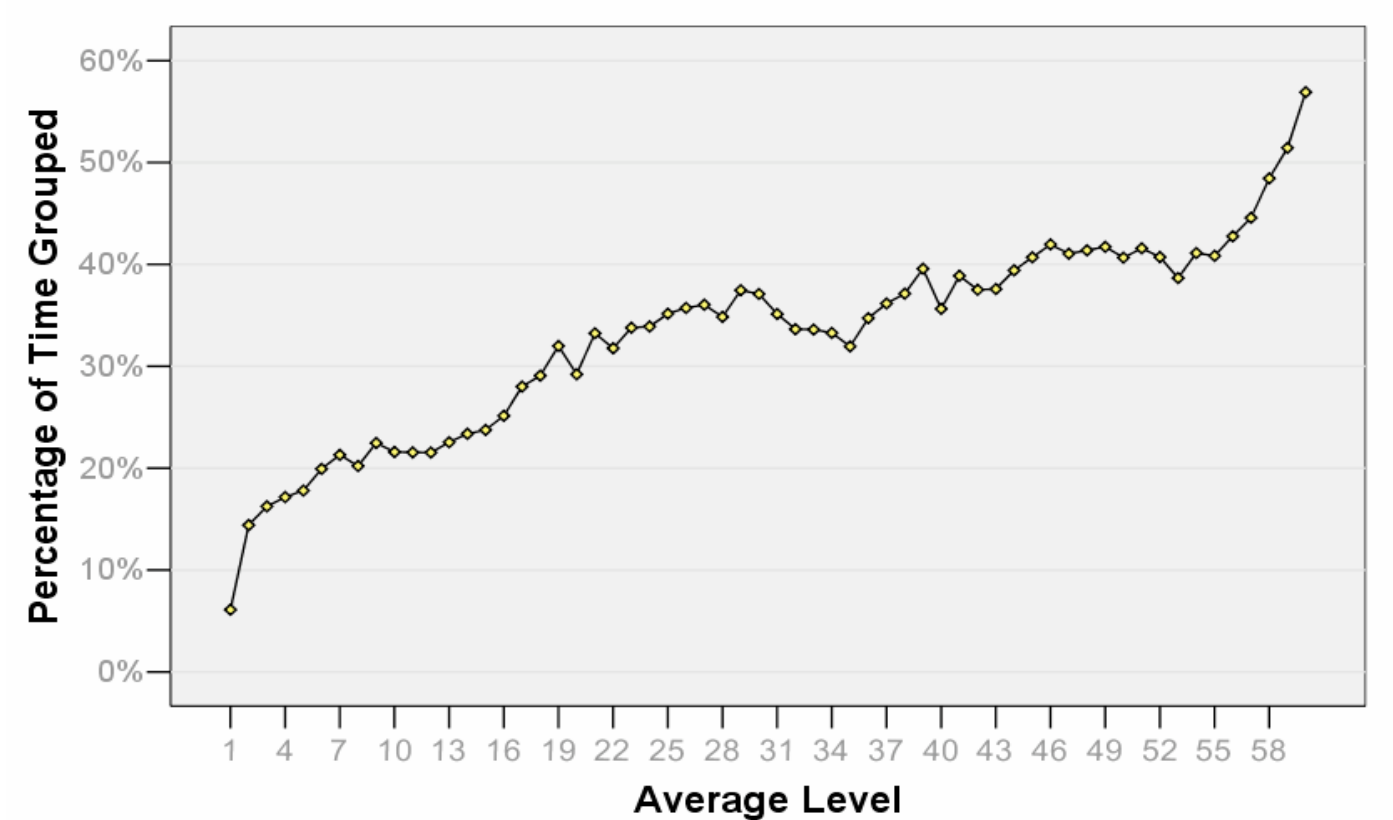
\includegraphics[scale=0.95]{./images/timespentgroup.png}
        \caption{Temps moyen passé en groupe, par classe}
        \label{timespentgroup}
        \end{figure}

\subsection{Jouer en guilde}
World Of Warcraft encourage les joueurs à former des groupes en utilisant deux mécanismes. Premièrement, pour qu'une complémentarité entre les habilitées des joueurs se crée. Deuxièmement, beaucoup de quêtes dans le jeux sont difficiles à réaliser tout seul. Nous pouvons aussi voir que des différences se dégagent entre le temps passé an groupe en fonction de chaque espèce (voir figure~\ref{tabltimegroup}.
\par Ces groupes sont appelés des guildes, elles sont un des aspects de la popularité de ce type de jeu. Dans World Of Warcraft, 66\% des avatars appartiennent à une guilde et que ce chiffre atteint 90\% si l'on tient compte que des joueurs ayant au moins le 43. Les joueurs appartenant à une guilde joue en moyenne plus souvent qu'un joueur sans guilde. 
	\begin{figure}[!h]
        \centering
        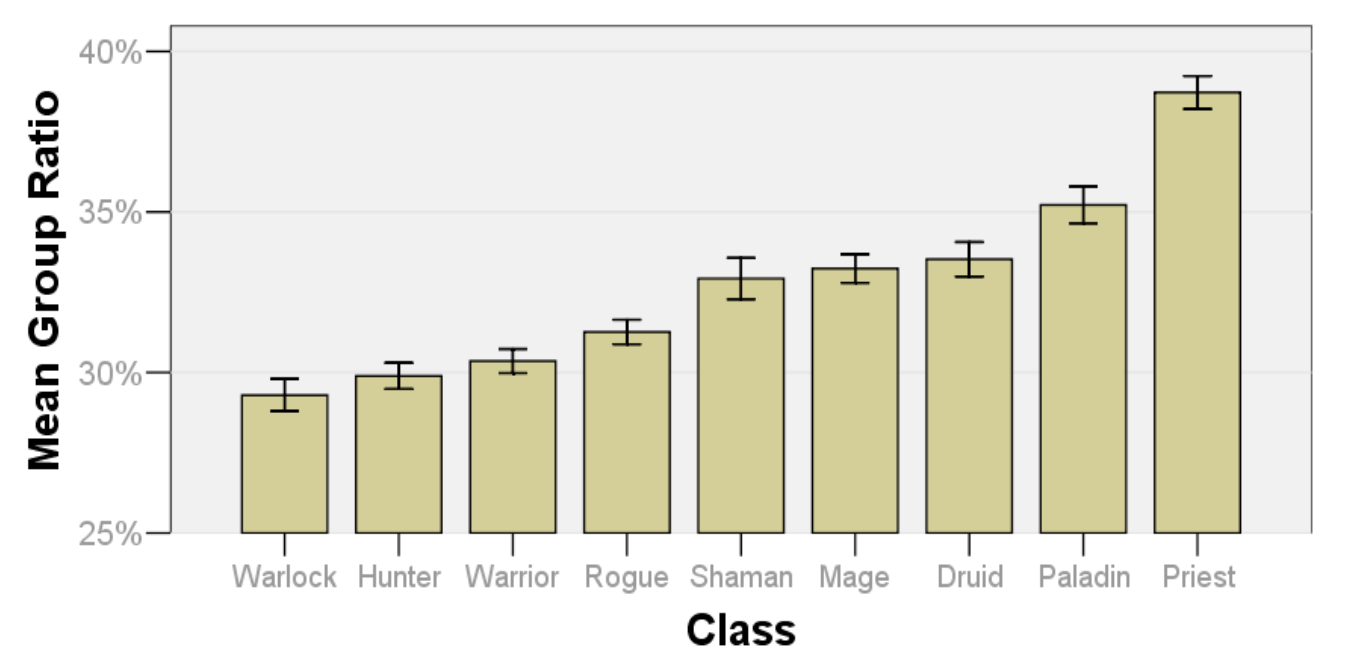
\includegraphics[scale=0.95]{./images/tabltimegroup.png}
        \caption{Temps moyen passé en groupe, par classe}
        \label{tabltimegroup}
        \end{figure}
\par Un des facteur important, pour essayer de réaliser un modèle de mobilité, est d'étudier la taille des guildes. La moyenne de personne dans une guilde est de 14,5\% (16,8\% si l'on exclut du calcul les guildes de une personne). Le median est de 6 (9 si l'on exclut du calcul les guildes de une personne). 

\subsection{Social Networks} 
\newpage
\section{The changing Dynamic of Social Interaction in World of Warcraft}



\newpage
\bibliographystyle{plain}
\bibliography{Biblio}


 

\end{document}

